\documentclass{article}
\usepackage[utf8]{inputenc}

\title{Rethinking the Inception Architecture for Computer Vision}
\author{}
\date{}

\usepackage{natbib}
\usepackage{graphicx}
\usepackage{amsmath}
\usepackage[left=2.5cm,right=2.5cm,top=1cm,bottom=1.25cm]{geometry}
\usepackage{hyperref}
\usepackage{float}
\usepackage[export]{adjustbox}



\hypersetup{colorlinks=true,urlcolor=blue}
\pagenumbering{gobble}

\begin{document}

\maketitle

\section*{Link}
\href{https://arxiv.org/abs/1512.00567}{arXiv} 

\section*{Summary}
\begin{itemize}
    \item The paper proposed several design principles for deep CNNs
    \begin{enumerate}
        \item Avoid representational bottlenecks, especially early in the network. The representation size should gently decrease from input to the output.
        \item Having higher dimensional representations allow for more disentangled features and faster training.
        \item Before performing more spread out convolution(e.g. $3 \times 3$) one can reduce the dimension of the input representation before spatial aggregation without expecting serious adverse effects. This is probably because of strong correlation between adjacent units which results in much less loss of information during dimension reduction.
        \item Optimum performance of the network can be obtained by balancing the number of filters per stage and the depth of the network.
    \end{enumerate}
    \item Convolution with large kernel size can be factorized for efficiency. This can be accomplished in two ways
    \begin{enumerate}
        \item Factorize large convolution into sequence of smaller convolutions. For example replacing a $5\times5$ convolution with two $3\times 3$ convolution results in computational saving of $(3\times 3+3 \times 3)/(5\times 5)$ or 28\% but preserves the effective receptive field. Using non-linear activation in the intermediate layers improve performance. There is no significant drop in performance due to this form of factorization. 
        \item Convolution can also be factorized asymmetrically. A $n\times n$ convolution can be factored into one $1\times n$ convolution followed by a $n \times 1$ convolution. For example by replacing $3\times 3$ convolution with $1 \times 3$ and $3 \times 1$ convolution we can reduce computation by $(3+3)/(3\times 3)$ or 33\%. However this does not work well on early layers but gives very good result on medium sized grids where very good results can be obtained by using $1\times 7$ convolution followed by $7 \times 1$ convolution.  
    \end{enumerate}
    \item Using auxiliary classifiers did not result in improved convergence early in the training but during the end of the training they achieved slightly higher accuracy.
    \item To reduce grid size efficiently we can two parallel blocks, one convolutional and one pooling, both of stride 2 and then concatenate them.  
    \begin{figure}[H]
        \centering
        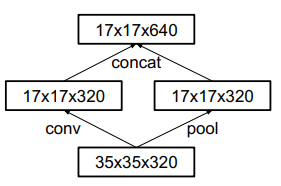
\includegraphics[scale=0.75]{grid_reduction.PNG}
        \caption{Efficient grid size reduction}
        \label{fig:Figure 1}
    \end{figure}
    \item When we use cross entropy loss with one hot target labels, it is equivalent to maximizing the log-likelihood of the correct labels. It may result in overfitting. If the model assigns full probability to the correct label it won't be able to generalize well. They propose a mechanism called label-smoothing regularization(LSR) to make the model less confident about its output. Specifically they replace the label distribution $q(k|x)=\delta_{k,y}$ with $q'(k)=(1-\epsilon)\delta_{k,y}+\dfrac{\epsilon}{K-1}$ with $\epsilon = 0.1$. This means now the probability of wrong labels will be penalized if they are too small. This approach resulted in 0.2\% gain in absolute accuracy.
    \item They used RMSprop with weight decay 0.9 and decaying learning rate. The gradient were clipped at 2.0 threshold.
    \item When computational cost is kept constant it is more difficult to train lower resolution images and the accuracy is also slightly lower. Naively reducing size of the network according to input resolution will result in a network that performs much more poorly because the task of recognizing lower resolution image is more difficult. 
\end{itemize}
\end{document}
